\newpage
\appendix
\section{Succinct Data Structures}



\subsection{Functionality of Rank \& Select}\label{App:rank_select}
Let \(B\) be a sequence of \(n\) items. Then \textbf{rank(c)} and \textbf{select(c)} can be defined as:
\begin{description}
  \item[rank(o)] 
  Counts the number of items which appear in \(B\) from its start to its o-th position \cite{Jacobson89}.
  \item[select(o)]
  Finds the o-th occurrence of an element in \(B\) \cite{Jacobson89}.
\end{description}

The time complexity of rank/select queries depends on the structure where these two operation are built on. For example, it is possible to execute rank/select in constant \(\mathcal{O}(1)\) time for some bit-vectors, like rrr-vectors \cite{Raman}, or another binary rank index \cite{dillabaugh_2007}.

\subsection{Wavelet Trees} {\label{App:WT}}
Wavelet Tree (introduced by \citeauthor{Grossi} \citeyear{Grossi}) organises a string into a bit-vector hierarchy with a space complexity of \(\mathcal{O}(N\log_2\sigma)\). The time complexity of a rank query is \(\mathcal{O}(\log_2\sigma)\) with \(\sigma\) to be the size of the alphabet of the string \cite{bowe_2011} and $N$ its length.

\subsubsection{Construction of a Wavelet Tree}
Having a sequence of symbols, for simplicity reasons it will assumed that it is a string, a wavelet tree converts that string into a balanced binary tree of bit vectors. Half the symbols of the string are replaced with 0 and the other half with 1. It is clear though that this representation creates ambiguity. That is why at each level of the tree, the remaining alphabet is filtered and is re-encoded as a result the ambiguity lessens, until the point that on the final level of the tree there is no ambiguity at all \cite{bowe_2011}.
As shown in Figure \ref{fig:WT}, the alphabet of the phrase "Peter Piper picked a peck of pickled peppers" is \{\$,P,\_,a,c,d,e,f,i,k,l,o,p,r,s,t\}. The first half of the alphabet is mapped to 0 and the rest to 1 and each half of the mapped bits is stored to two bit vectors which constitute the first level of the wavelet tree. The left bit vector is created by taking the symbols mapped under 0 and the right bit vector by taking the symbols mapped under 1. The same procedure follows for each branch of the tree.

\begin{figure}[h]
    \centering
    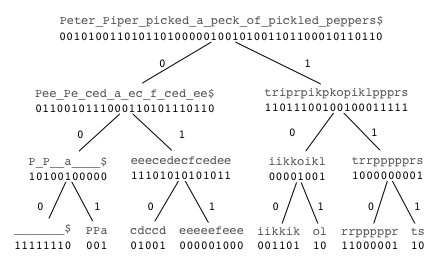
\includegraphics[width=0.5\textwidth]{binwt}
    \caption{Wavelet tree for the string "Peter Piper picked a peck of pickled peppers" (spaces and a string terminator have been represented as \_ and \$ respectively. The strings are not stored; just shown for convenience reasons}
    \label{fig:WT}
\end{figure}

\subsubsection{Querying a Wavelet Tree}
Having constructed the wavelet tree, a rank query can be done in \(\log_2\sigma\) time. An example of a rank\textsubscript{e}(5) query is shown in Figure \ref{fig:WT_Q}, where symbol e is tracked downwards the wavelet tree. A similar procedure could be done in case it was needed to track a symbol upwards (starting from a leaf, e.g.\ select\textsubscript{e}(5)).
\par From the first level of the tree we know that e is encoded as 0. Doing a rank query of 0 at this level, it is returned the position where the next rank should be done on the 0-child. The next rank should be a query of 1 since at this level e is now encoded as 1. This procedures continues recursively, until a leaf of the tree is reached and any ambiguity is lost, giving a reply to the rank query. 

\begin{figure}[h]
    \centering
    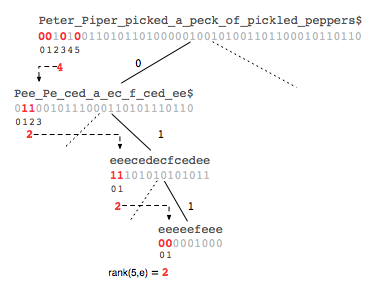
\includegraphics[width=0.5\textwidth]{binwt-query}
    \caption{Recursive repetition of a rank query in a wavelet tree}
    \label{fig:WT_Q}
\end{figure}


\newpage
\section{Burrows-Wheeler Transform} \label{App:BWT}
The Burrows-Wheeler Transform (BWT), developed by Burrows and Wheeler, as a way to reversibly permute a string in such a way that characters from repeated substrings would be clustered together \cite{adjeroh_bell_mukherjee_2008, bowe_2011_FM}. It is useful for compression schemes such as run-length encoding.
\par BWT is performed to a sequence of characters through rotations among the sequence’s characters. The number of the rotations equals the length of the sequence minus one. After all the rotations, Figure \ref{fig:bwt} (a), the rotation list is sorted in order the result of BWT to be obtained. The last column (\(L\)), in this example is (k, \$, a, v, r, r, a, a, d), is essential because the first column (\(F\)) can be produced from sorting \(L\) while the pair for each character from the last column and first column gives what character comes before another consecutively. Hence, all the pairs \(\langle L[a], F[a] \rangle\) are consecutive characters in the sequence \cite{adjeroh_bell_mukherjee_2008}.

\begin{figure}[h]
    \centering
    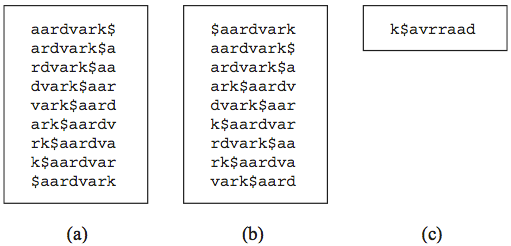
\includegraphics[width=0.5\textwidth]{bwt}
    \caption{Burrows-Wheeler Transform of the string “aardvark\$”: (a) all rotations of the text are listed; (b) the list is sorted; (c) the last column is extracted as the BWT output \cite{adjeroh_bell_mukherjee_2008}}
    \label{fig:bwt}
\end{figure}

\subsection{Suffix Arrays}
In a simple form, a suffix array SA[1..N] can be constructed by the following steps \cite{Puglisi}.
\begin{enumerate}
	\item Construct an array of pointers to all suffixes S[1..N], S[2..N], \ldots, S[N..N].
	\item Sort these pointers by a lexicographical (i.e.\ alphabetical) order of their corresponding suffixes.
\end{enumerate}

The Figure \ref{fig:sa} shows a trivial example of the world "mississippi" where \$ is the terminating character. There are several construction algorithms of suffix arrays including some ones with \(\mathcal{O}(N)\) complexity.

\begin{figure}[h]
    \centering
    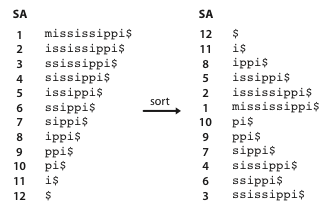
\includegraphics[width=0.5\textwidth]{mississippi-sa-sort}
    \caption{Suffix Array creation of the word "mississippi"}
    \label{fig:sa}
\end{figure}

Having now a suffix array as a tool, it can be used as a way to easily output the BWT of a string S. Specifically, the transform can be calculated through: BWT[a]=S[SA[a]–1, BWT[1]=\$ (terminating character \$ since BWT wraps around). A simple example is shown in Figure \ref{fig:bwt_sa}.

\begin{figure}[h]
    \centering
    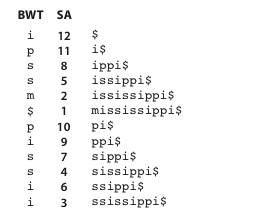
\includegraphics[width=0.4\textwidth]{mississippi-sa}
    \caption{BWT of the world "mississippi" through a suffix array}
    \label{fig:bwt_sa}
\end{figure}


\subsection{FM-Index}
\citeauthor{Ferragina} \citeyear{Ferragina} suggested that a BWT be paired with a suffix array creates the so called \emph{FM-Index}. With the FM-Index it is possible to get reconstructed the original string allowing to discard the original document. Hence any given information that has been transformed through BWT can be reversible \cite{Ferragina}.
\subsection{Backward Search on FM-Index}{\label{App:bs_fm}}
Substring search can be certainly considered as a wide reaching problem. Recent applications on this problem like genome assembly has been studied by \citeauthor{3_simpson_durbin_2010} \citeyear{3_simpson_durbin_2010}. Tools like the aforementioned ones (secionts \ref{App:SDS} and \ref{App:BWT}) can be combined together creating in that way a powerful tool. \emph{Backward Search} can be considered as such a tool (Figure \ref{fig:overview_sds_bwt_sa}).

\begin{figure}[h]
    \centering
    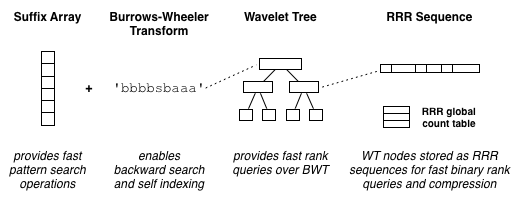
\includegraphics[width=0.75\textwidth]{overview_SA_BWT_WT_RRR}
    \caption{An overview of Succinct Data Structures combined with BWT and Suffix Array to efficiently enable Backward Search}
    \label{fig:overview_sds_bwt_sa}
\end{figure}

Backward search utilises the BWT in a series of paired rank queries (e.g.\ a wavelet tree can efficiently provide such functionality), offering a considerably  good performance in queries where occurrences of a pattern are searched in a string. Let us consider a pattern \(P\) and a sequence/string \(S\). With backward search will be done \emph{p} pairs of rank queries in order to get the location of all the occurrences of \(P\) in \(S\), where p is the length of the pattern. The paired rank queries are as follows \cite{Ferragina}:

\[s\prime = C[P[a]] + rank_{s-1}(P[a])+1\]
\[e\prime = C[P[a]] + rank_{e}(P[a])\]

Where \(s\) is the start of the range (regarding the sequence \(S\)) and \(e\) is the end of it. A count table for all the symbols of the alphabet is \(C\). The count table refers to the symbols of \(S\) in a lexicographic order. Backward search is named that way because when the search of a patter is started, the initial value of \(a\) is \(\vert P \vert\). Hence, the search is started from the last symbols of the pattern and continues backwards  by decreasing \(a\) every time by 1.  If at any stage \(e<s\), then \(P\) does not exist in \(S\). The reason which that happens depends on the fact that SA[\(s\ldots e\)] contains all the suffixes of which \(P[a \ldots \vert{P}]\) is a prefix, and as a result all the locations of it.
\subsubsection{Backward Search Complexity}
As stated in Section \ref{App:bs_fm}, a backward search in order to get completed (and discover the occurences of a pattern) needs p pairs of rank operation calls. This attribute remains the same regardless the size of $S$. Hence, the overall complexity to find all the occurences of a pattern of size p is p\(\times\mathcal{O}(\log_2\sigma)\) with $\sigma$ to be the alphabet size of $S$. Hence, the fact that the speed of the algorithm is independent of the training input size makes it more or less scalable enough. Especially if it is taken into account that the main drawback of an algorithm could be that it gets slower and slower as the input data that it processes gets larger and larger. Having an algorithm that its speed is not affected by this aspect is crucial.
\par In addition, the required space needed to represent $S$ (or any training input) and perform backward search on it, is the space needed to store $S$ in a wavelet tree with the additional space needed for the count table $C$ which is \(\mathcal{O}(\sigma)\). Most of the times it is used even less space in comparison of the same input stored to a file in a disk or space very close to the information theoretic lower bound  \cite{ktistakis}

\subsubsection{Backward Search Example}{\label{bs-ex}}
In Figure \ref{fig:bs_stages}, it is shown all the stages for locating the occurrences of pattern "iss" in the string "mississippi". Backward search starts with \(a=3, c=P[a]=\text{\lq{s}\rq}\) and the first pair of ranks is:
\[s\prime = C[c] + rank_c(0) + 1 = 8+0+1=9\]
\[e\prime = C[c] + rank_c(12) = 8+4=12\]

After that stage, it continues with the next pair of ranks:
\[a=2,s=9, e=11, c=P[a]=\text{\lq{s}\rq}\]
\[s\prime\prime = C[c] + rank_c(8) + 1 = 8+2+1=11\]
\[e\prime\prime = C[c] + rank_c(12)= 8+4=12\]

and finally:

\[s\prime\prime\prime = C[c] + rank_c(10) + 1 = 1+2+1=4\]
\[e\prime\prime\prime = C[c] + rank_c(12)= 1+4=5\]

All the occurrences of "iss" lie in SA[4\ldots 5].


\begin{figure}[h]
    \centering
    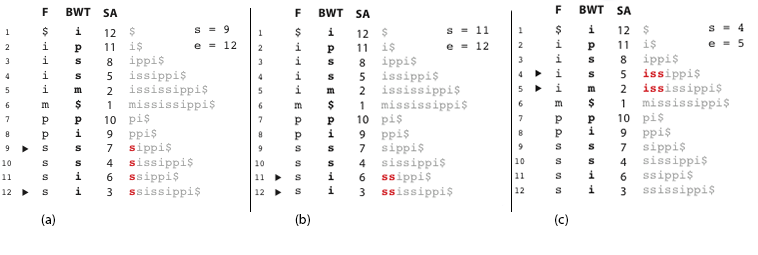
\includegraphics[width=0.8\textwidth]{bs_stages}
    \caption{The three stages of backward search described in Section \ref{bs-ex}}
    \label{fig:bs_stages}
\end{figure}

\subsection{Document Listing using Backward Search}{\label{App:bs_doclist}}
Having a set of sequences, it is a usual problem that we may want to search for a pattern among those sequences and simultaneously retrieve the sequences that contain the searched pattern. The sequences can otherwise described as documents. Hence, the problem lies on the fact of listing documents containing a specific pattern. It is possible to solve document listing problem using backward search on FM-Index. A way of doing that is through the construction procedure of a suffix array. When a pattern is searched in a dataset, in order to find the occurrences of the pattern in the dataset, it is important to concatenate all the sequences (documents) in one long string. For this one string, it is created the suffix array and a backward search is applied. Now, for listing the documents that the pattern occurs, we need an array that stores which sequence the pointed suffix from the suffix array belongs to. An example is show in Figure \ref{fig:doc_list}. The first position of suffix array points to ``D". Since this suffix belongs to the first sequence, the array of documents will hold the number one on the same position. The same happens for the rest of suffixes. When the suffix array is being sorted, the array containing the documents is simultaneously sorted with the same order. At the point the backward search is performed, and a range with the occurrences of a pattern is returned, the same range applies for the array containing the relative documents. Let us search for the pattern ``o" in Figure \ref{fig:doc_list}; the range SA$[17,\ldots,18]$ contains the occurrences of ``o". Then, the sequences containing the same pattern are the D$[17,\ldots,18]$. 
\par This combination of these two structures, gives the opportunity of creating efficient algorithms where the fact of obtaining sequences containing a pattern is important. The time complexity is not increased in comparison to backward's search complexity while the space complexity is slightly increased according to space need to store the references to the number of documents/sequences in D array.

\begin{figure}[h]
    \centering
    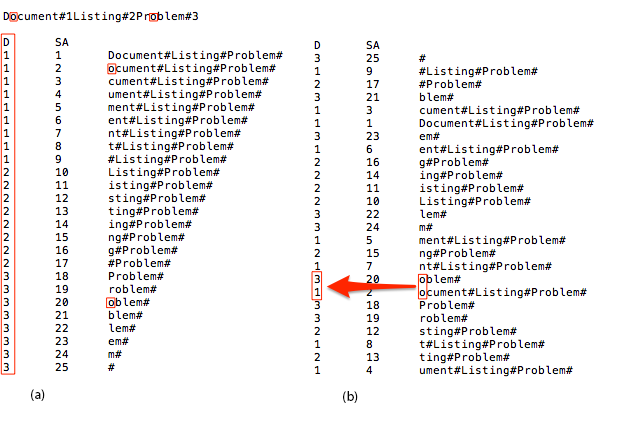
\includegraphics[width=0.8\textwidth]{doc_list}
    \caption{(a) Suffix Array with D array (documents) where every suffix begins (b) Simultaneously sorting Suffix Array and D }
    \label{fig:doc_list}
\end{figure}



